\chapter{Estado de la Cuestión}
\label{cap:estadoDeLaCuestion}
% En el estado de la cuestión es donde aparecen gran parte de las referencias bibliográficas del trabajo. Una de las formas más cómodas de gestionar la bibliografía en {\LaTeX} es utilizando \textbf{bibtex}. Las entradas bibliográficas deben estar en un fichero con extensión \textit{.bib} (con esta plantilla se proporciona el fichero biblio.bib, donde están las entradas referenciadas más abajo). Cada entrada bibliográfica tiene una clave que permite referenciarla desde cualquier parte del texto con los siguiente comandos:

% \begin{itemize}
% \item Referencia bibliografica con cite: \cite{ldesc2e}
% \item Referencia bibliográfica con citep: \citep{notsoshort}
% \item Referencia bibliográfica con citet: \citet{latexAPrimer}
% \end{itemize}

% Es posible citar más de una fuente, como por ejemplo \citep{latexCompanion,LaTeXLamport,texKnuth}

% Después, \LaTeX se ocupa de rellenar la sección de bibliografía con las entradas \textbf{que hayan sido citadas} (es decir, no con todas las entradas que hay en el .bib, sino sólo con aquellas que se hayan citado en alguna parte del texto).

% Bibtex es un programa separado de latex, pdflatex o cualquier otra cosa que se use para compilar los .tex, de manera que para que se rellene correctamente la sección de bibliografía es necesario compilar primero el trabajo (a veces es necesario compilarlo dos veces), compilar después con bibtex, y volver a compilar otra vez el trabajo (de nuevo, puede ser necesario compilarlo dos veces). 

En este capítulo se muestran las conclusiones obtenidas de la investigación previa a la implementación de la herramienta, es importante para situarse en los conocimientos y técnicas que existen para el fin de esta.

\section{Codificación y decodificación de imagen y audio}
En esta sección se describirán los procesos de codificación y decodificación de imagen y audio, específicamente en los formatos PNG y WAV. Estos formatos han sido seleccionados porque son los utilizados en la herramienta, ya que ambos garantizan la preservación de los datos originales al ser formatos sin pérdida.

\subsection{Imagen}
La codificación de imágenes en el formato PNG (\textit{Portable Network Graphics}) consiste en convertir datos visuales en un archivo digital comprimido sin pérdida de calidad. Este formato, desarrollado en 1996, soporta imágenes de color indexado, en escala de grises y de color de alta calidad (hasta 16 bits por píxel), además de un canal opcional alfa para corrección de color o transparencia. Según describe \cite{renau2011}, el proceso utiliza el algoritmo Deflate, que combina la compresión LZ77 y la codificación Huffman, creado por Phil Katz en 1996 para PKZIP\footnote{PKZIP es un software de compresión de archivos desarrollado por PKWARE, introdujo el popular formato de compresión de archivos ZIP.} y adoptado como base de la compresión PNG. Durante la codificación, los píxeles se comprimen con una tasa alta (superior a la de GIF [\textit{Graphics Interchange Format}]) mediante este método sin pérdidas, lo que permite almacenar la imagen eficientemente mientras se mantiene toda su información original. PNG también ofrece visualización progresiva, similar a GIF y JPEG (\textit{Joint Photographic Experts Group}), y destaca por su robustez ante errores de transmisión, siendo ideal para internet.\\

Internamente, un archivo PNG se representa como una matriz de píxeles, donde cada píxel está compuesto por valores que representan los colores en formato RGB (\textit{Red, Green, Blue}) o, en su caso, en escala de grises. En imágenes en color, cada píxel tiene tres valores, uno por componente RGB, y si incluye transparencia, un cuarto valor correspondiente al canal alfa. Cada uno de estos valores de color generalmente se representa con 8 bits (0-255), sumando 24 bits por píxel en imágenes RGB, y 32 bits si incluye alfa.
\begin{figure}[h]
	\centering
	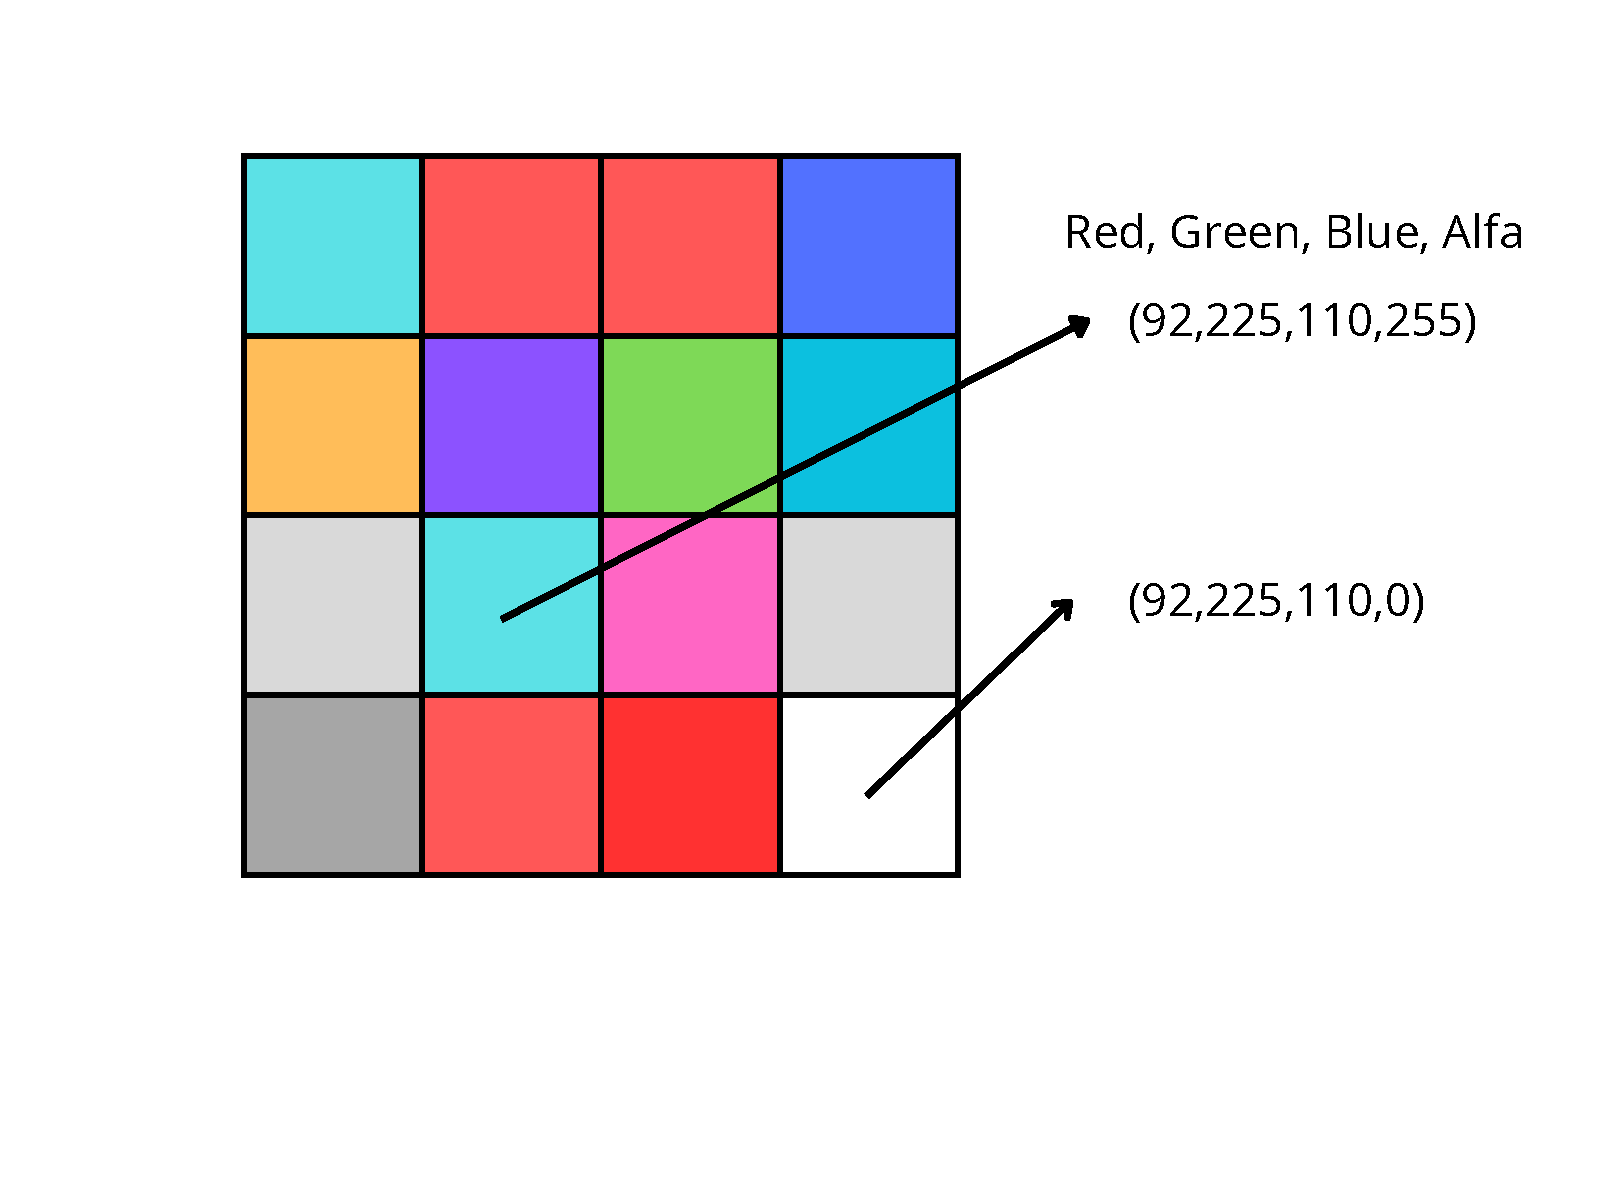
\includegraphics[width = 0.7\textwidth]{Imagenes/pitea/PNG.pdf}
	\caption[Representación de una imagen en formato PNG.]{Representación de una imagen en formato PNG. Elaboración propia.}
	\label{fig:proceso}
\end{figure}


La decodificación de una imagen PNG implica revertir este proceso: el archivo comprimido se descomprime usando el algoritmo Deflate, reconstruyendo los datos de los píxeles exactamente como estaban antes de la codificación. Dado que es un formato sin pérdidas, no se descarta información, y la imagen resultante es idéntica a la original, ya sea en color, escala de grises o con canal alfa. Este formato, diseñado como estático (a diferencia de su variante animada MNG [\textit{Multiple-image Network Graphics}]), garantiza que la visualización final preserve la calidad y las características del archivo codificado.

\subsection{Audio}
\label{sec:audioo}
La codificación de audio en el formato WAV (\textit{Waveform Audio File Format})  consiste en convertir una señal sonora analógica en un archivo digital sin pérdida de datos. Según \cite{MicrosoftIBM1991}, WAV es un formato que se utiliza para almacenar flujos digitales de audio y emplea principalmente LPCM como codec (\textit{Linear Pulse Coded Modulation}, Modulación por impulsos codificados lineal, no comprimido), el cual no tiene pérdida de calidad. Este proceso digitaliza el audio mediante un muestreo de la señal a una frecuencia como 44100 Hz (calidad de CD) y cuantificando cada muestra con una profundidad de 16 bits por cada canal de audio, almacenando estas muestras sin compresión. El archivo WAV incluye un encabezado que especifica múltiples datos de canales de audio como la frecuencia de muestreo, el número de canales (mono o estéreo) y la profundidad de bits, seguido de los datos de audio, lo que lo hace adecuado para uso profesional y para la herramienta donde se requiere máxima fidelidad.\\


Internamente, un archivo WAV representa el audio como una serie de muestras de amplitud tomadas en intervalos regulares (frecuencia de muestreo). Cada muestra corresponde a la amplitud de la señal en ese momento específico, y se representa como un valor binario. El formato WAV puede ser mono o estéreo, dependiendo del número de canales. En un archivo estéreo, cada muestra tiene dos valores (uno para el canal izquierdo y otro para el derecho). La frecuencia de muestreo determina cuántas muestras se toman por segundo, mientras que la profundidad de bits define la precisión de cada muestra.
\begin{figure}[h]
	\centering
	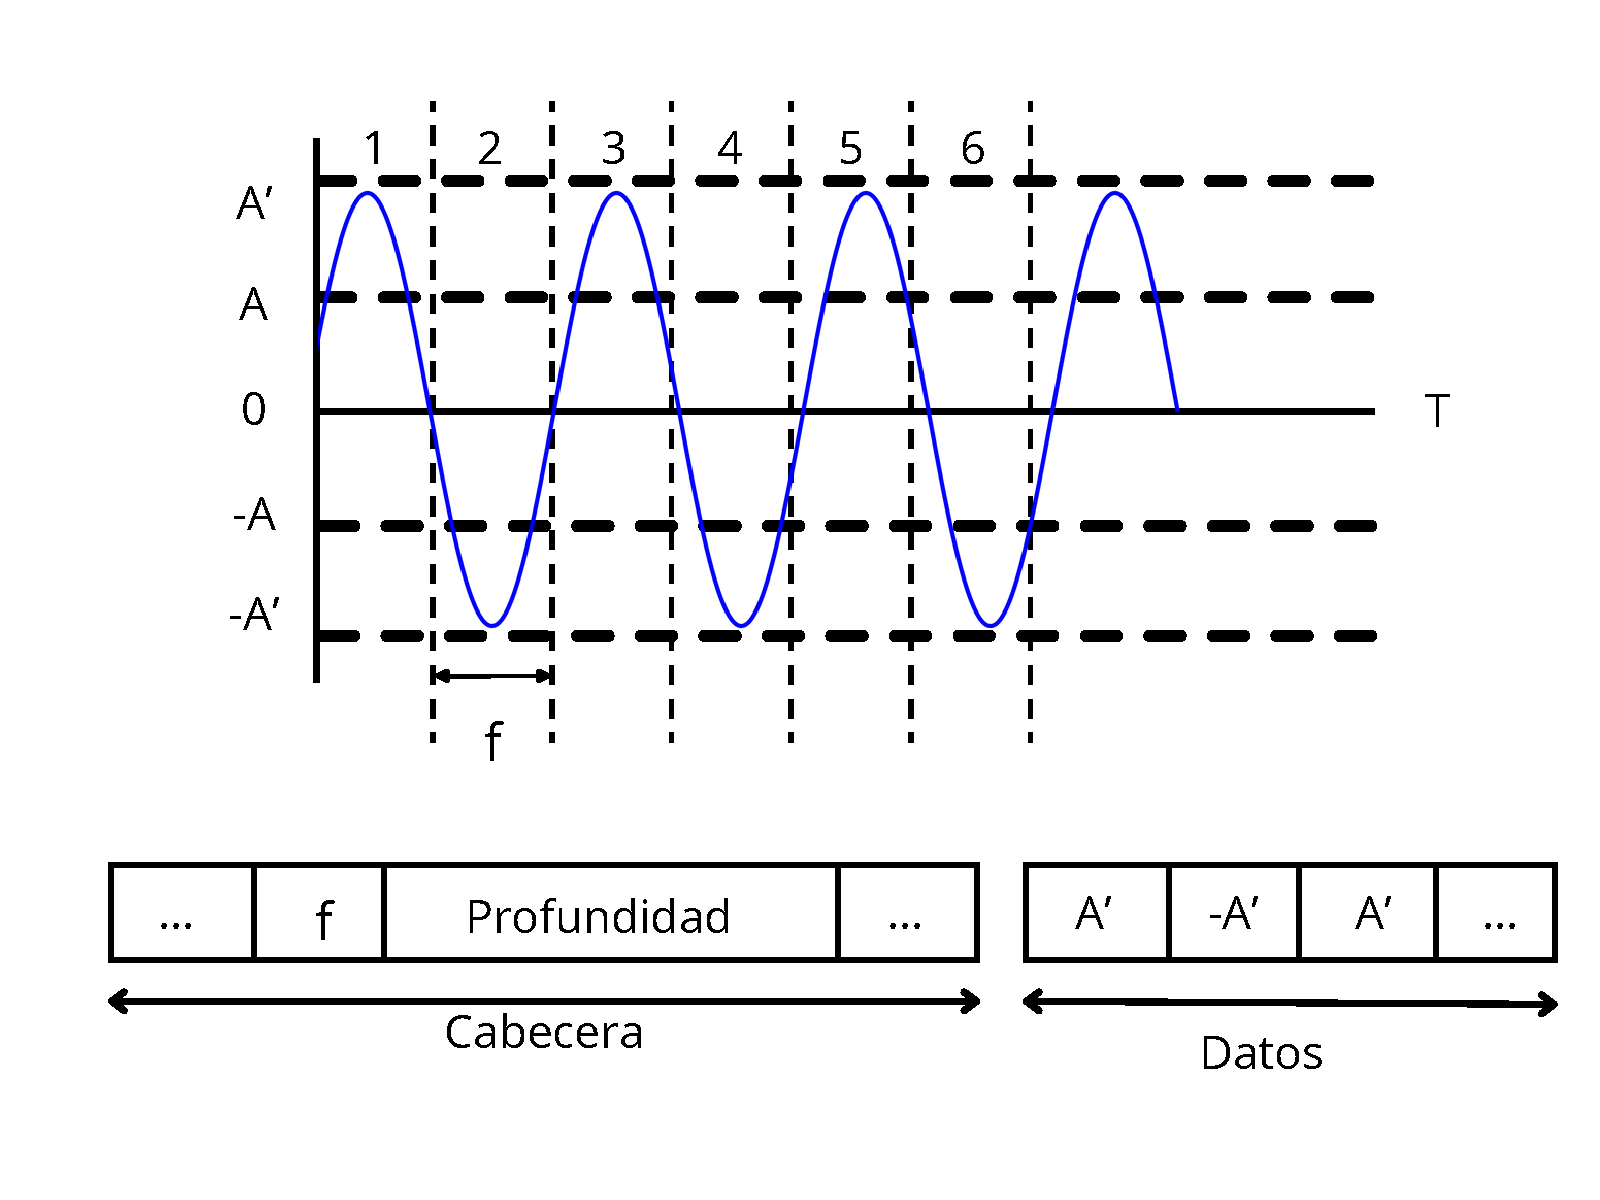
\includegraphics[width = 0.85\textwidth]{Imagenes/pitea/wav.pdf}
	\caption[Representación de un audio estéreo en formato WAV.]{Representación de un audio estéreo en formato WAV. Elaboración propia.}
	\label{fig:proceso2}
\end{figure}

La decodificación de un archivo WAV consiste en leer las muestras digitales almacenadas y convertirlas nuevamente en una señal sonora reproducible. Según \cite{MicrosoftIBM1991}, el encabezado proporciona la tasa de muestreo (ejemplo, 44100 Hz) y la cantidad de bits por muestra (ejemplo, 16 bits), permitiendo a los programas interpretar las muestras LPCM no comprimidas para reproducir el audio con máxima calidad y sin pérdida de datos, como se requiere en la herramienta.

\section{Esteganografía}

En esta sección se hablará de la esteganografía, definiéndola, mencionándose su empleo a lo largo de la historia, tipos y sus usos en archivos multimedia.

\subsection{Orígenes}

Uno de los primeros ejemplos conocidos del uso de la esteganografía, según \cite{salas2015}, se remonta  aproximadamente a 400 años antes de Cristo en la Antigua Grecia. Un personaje cogió dos tablillas cubiertas de cera, las cuales solían ser rayadas en la superficie como método de escritura, además grabó un mensaje en la madera de las tablillas antes de cubrirlas, quedando oculto bajo la cera y siendo solo posible leerse tras derretirla. En esta historia, el conjunto de las tablillas y la cera funcionaba como un archivo ``inocente'', mientras que el mensaje real permanecía oculto bajo capas de cera.\\



Otro ejemplo histórico, estrechamente ligado a la literatura española, es el caso de \textit{La Celestina}, escrita alrededor de 1485 y publicada en 1499. En esta obra, su autor, en un principio anónimo, ocultó su nombre en las primeras letras de los versos del preámbulo de la obra, dejando así su firma a plena vista\footnote{Estos versos pueden encontrarse en \url{https://www.badosa.com/bin/obra.pl?id=n266-02}.}.
Esta misma técnica, según \cite{salas2015}, fue utilizada en \textit{El sueño de Polífilo (Hypnerotomachia Poliphili)} de Francesco Colonna, publicado en 1499. En este caso, la primera letra de cada capítulo forma el mensaje ``\textit{Poliam frater Franciscus Columna peramavit}'', una declaración de amor en latín que, traducida al español, significa ``El hermano Francesco Colonna amó apasionadamente a Polia''.\\

Más recientemente, según~\cite{salas2015} tras la Segunda Guerra Mundial y la aparición de la informática, la esteganografía se volvió más refinada. Los servicios de inteligencia de varios países (CIA, Mossad, MI6, entre otros) comenzaron a darse cuenta de que los terroristas la utilizaban para comunicarse de manera oculta a lo largo de la red.  
Los analistas de los servicios secretos detectaron que usuarios relacionados con Al Qaeda empleaban el tablón de Reddit\footnote{\url{Https://www.reddit.com/} Reddit es una plataforma de discusión y agregación de contenido organizada en comunidades temáticas llamadas \textit{subreddits}.} para insertar anuncios aparentemente inocentes con caracteres hexadecimales y números primos, posiblemente utilizados como claves de cifrado para algoritmos como RSA. Sin embargo, no hay información confirmada sobre el propósito de la información oculta. Según un extracto de un libro publicado por \textit{The New York Post}, en más de una ocasión, Reddit habría permitido rastrear a terroristas que utilizaban este tipo de cifrado, cuyos mensajes, al ser decodificados, a veces indicaban la planificación inminente de un atentado, según~\cite{nyt2015}.




\subsection{Descripción}
Como define \cite{carracedo2004}, ``la esteganografía es la técnica y el arte de ocultar una información dentro de otra''. Según se menciona en su libro, esta disciplina ofrece un método simple para ocultar información mediante la aplicación de algoritmos que generan alteraciones imperceptibles en archivos que parecen inofensivos, como textos, imágenes o archivos de audio. Como resultado, se obtiene un archivo que alberga datos ocultos pero conserva la misma apariencia que el original, denominado comúnmente como archivo portador o inocente. Para recuperar el mensaje oculto, se aplica un proceso inverso al utilizado en la ocultación. 

\begin{figure}[h]
	\centering
	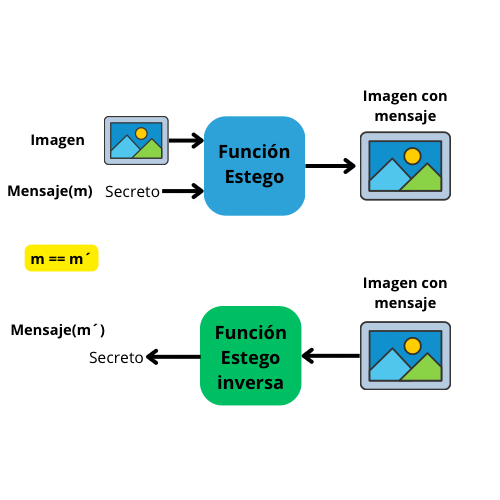
\includegraphics[width = 0.6\textwidth]{Imagenes/pitea/diagrama_estego.png}
	\caption[Diagrama de funcionamiento de la esteganografía.]{Diagrama de funcionamiento de la esteganografía. Elaboración propia.}
	\label{fig:proceso}
\end{figure}

\FloatBarrier  % Evita que la imagen pase más allá de este punto

\subsection{Tipos de esteganografía}

La esteganografía, como técnica para ocultar información, ha evolucionado a lo largo de los años, dando lugar a diversas clasificaciones y aplicaciones, tal como señala~\cite{PabloyIglesias}. A continuación, se presentan sus principales tipos y ámbitos de uso:

\begin{itemize}
  \item \textbf{Esteganografía pura:} Las técnicas de esteganografía pura se caracterizan por no emplear una estego-clave, la cual es una clave especial utilizada para determinar cómo y dónde ocultar o recuperar información en el archivo portador. Al no usar esta clave, el mensaje oculto se inserta directamente en el medio elegido sin necesidad de elementos adicionales. De este modo, se asume que un receptor no deseado será incapaz de reconocer que existe información oculta en un mensaje aparentemente normal, basándose así en un modelo de seguridad por oscuridad\footnote{Es un concepto que significa proteger información simplemente manteniendo en secreto el método utilizado para ocultarla o protegerla. }.
  
  \item \textbf{Esteganografía de clave secreta:} Por otro lado, en la esteganografía de clave secreta, la estego-función depende del uso de una clave conocida únicamente por el emisor y el receptor. Esta clave es fundamental, ya que determina la forma en la que el mensaje se camufla y cómo recuperarlo posteriormente. Un ejemplo simple sería utilizar una estego-clave para determinar la ubicación exacta dentro del archivo portador donde se comenzará a insertar el mensaje secreto.
\end{itemize}

~\cite{PabloyIglesias} señala que estas dos categorías abarcan una amplia variedad de aplicaciones, que incluyen su uso en textos, sistemas operativos, ficheros, formatos de archivo, hardware, tecnologías web, protocolos de comunicación y contenido multimedia en las cuales nos centraremos.\\

\subsection{Esteganografía en contenido multimedia}
Ocultar información dentro de archivos digitales, como imágenes o audios, aprovechando sus características para realizar modificaciones imperceptibles es en lo que consiste la esteganografía en contenido multimedia. Esta técnica permite almacenar datos adicionales sin alterar de forma significativa la calidad o la apariencia original del medio. Además, según  \cite{rodriguez2009esteganografia}, las técnicas de esteganografía  pueden clasificarse en dos grandes grupos: 
\begin{itemize}
    \item \textbf{Las basadas en el dominio de la imagen}: Estas técnicas ocultan la información modificando directamente los valores de los píxeles de la imagen. Generalmente son fáciles de implementar, aunque pueden ser vulnerables ante análisis forenses avanzados. Una de las técnicas más frecuentes es la sustitución de bits menos significativos (LSB, por sus siglas en inglés), que consiste en insertar información modificando los bits menos significativos de cada píxel. Este método también puede aplicarse en archivos de audio, modificando ligeramente sus muestras digitales para ocultar datos sin afectar perceptiblemente la calidad auditiva.

     \begin{figure}[h]
	\centering
	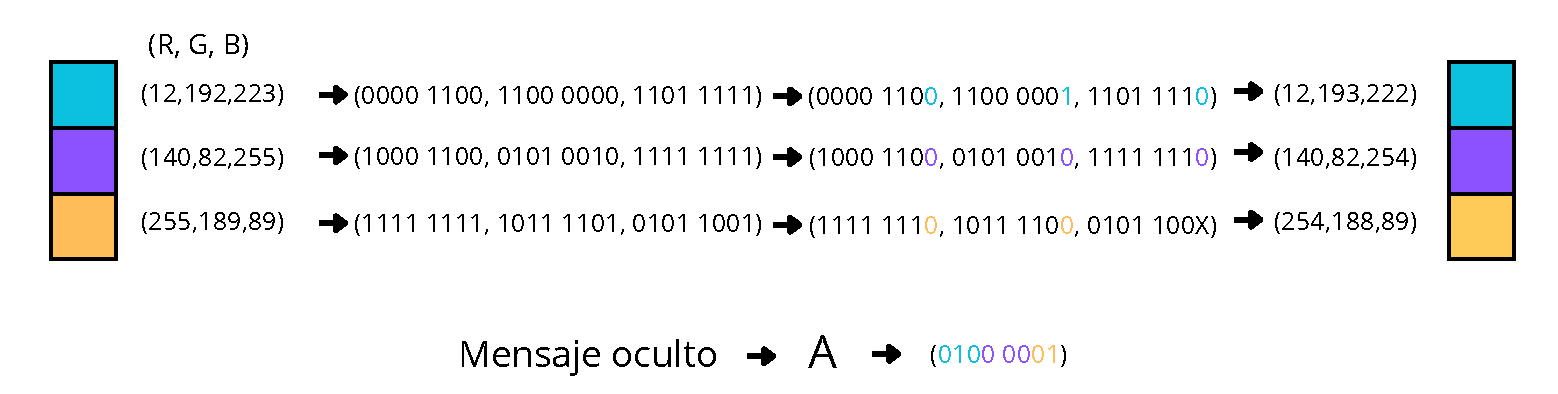
\includegraphics[width = 1\textwidth]{Imagenes/pitea/lsb_png.pdf}
	\caption[Ejemplo de LSB en una imagen PNG sin canal alfa.]{Ejemplo de LSB en una imagen PNG sin canal alfa. Elaboración propia.}
	\label{fig:proceso}
\end{figure}
    
    \item \textbf{Las basadas en el dominio de la transformación}: Estas técnicas utilizan algoritmos que modifican o transforman matemáticamente la imagen antes de insertar la información oculta, como se puede ver en la figura~\ref{fig:lsb_transformada}. Los mensajes suelen insertarse en las áreas más relevantes o significativas del archivo portador, aumentando así la resistencia ante modificaciones o análisis forenses y la probabilidad de que la información pueda sobrevivir a transformaciones. Además, pueden alterar propiedades específicas, como la luminosidad en imágenes, o ciertas características auditivas en el caso del audio.  Por ejemplo, en imágenes se suele utilizar la transformada discreta del coseno (DCT), la cual descompone la imagen en coeficientes de frecuencias. Luego, se modifica ligeramente alguno de estos coeficientes (normalmente aquellos menos perceptibles al ojo humano) para insertar el mensaje oculto. En audio, técnicas como el enmascaramiento auditivo aprovechan las limitaciones auditivas del oído humano para ocultar información en frecuencias o rangos que son poco perceptibles, o la técnica del eco, que consiste en insertar datos mediante la adición de ecos muy sutiles, imperceptibles para el oyente promedio. Estos enfoques, aunque más complejos, permiten una ocultación más resistente ante análisis forenses.

    \begin{figure}[h]
	\centering
	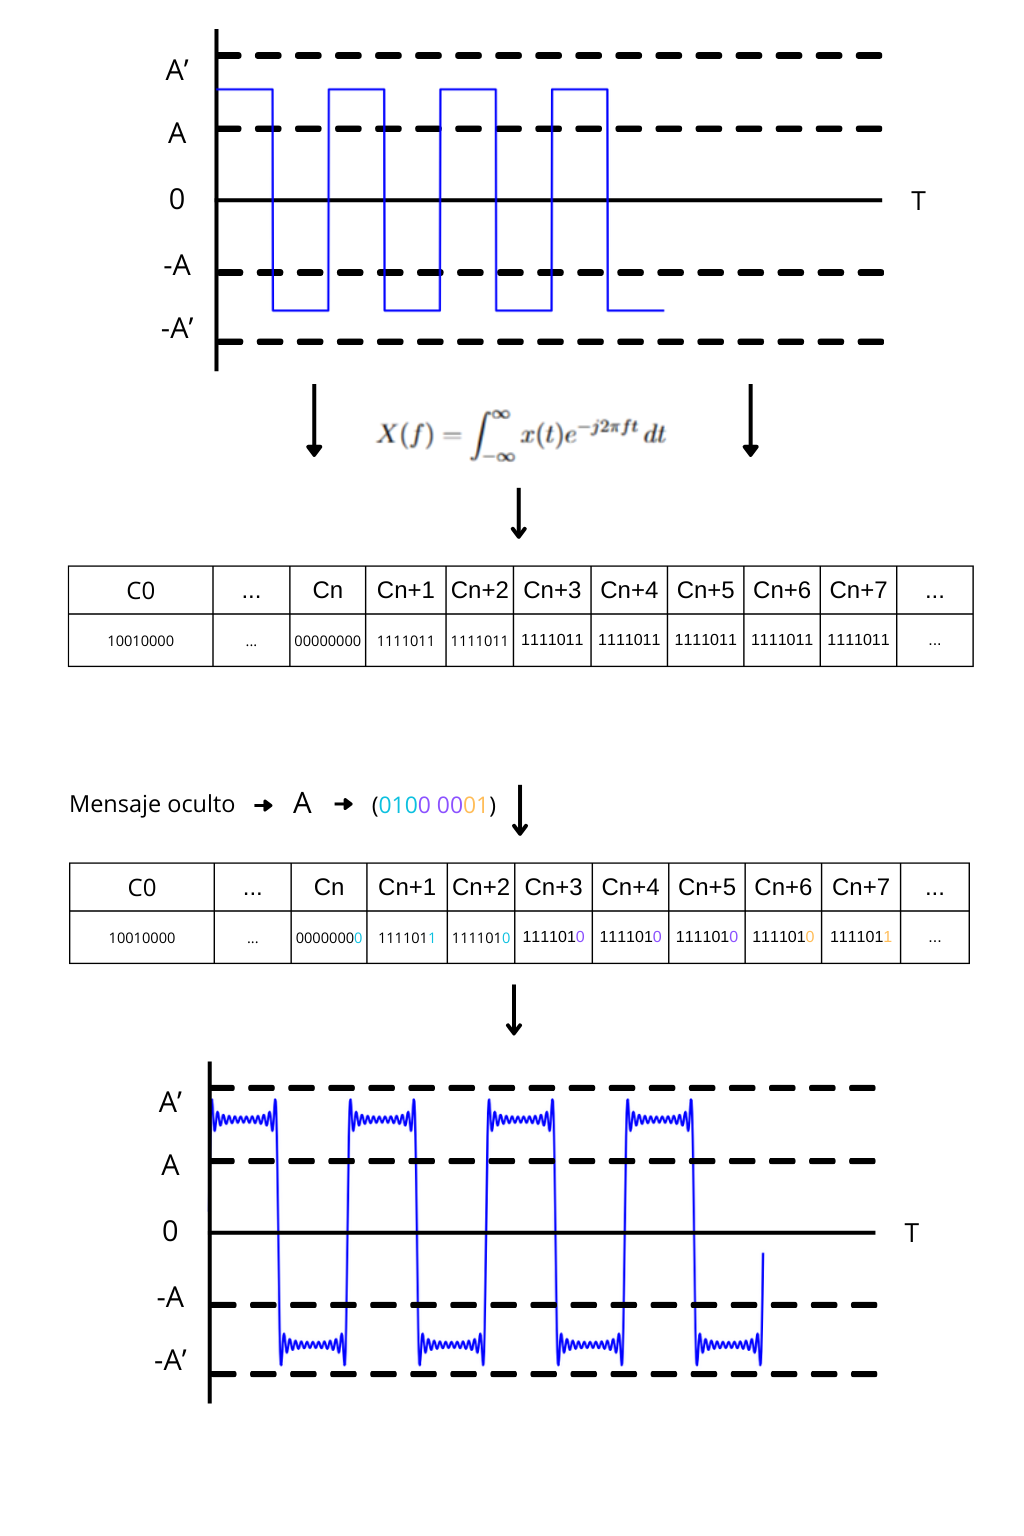
\includegraphics[width = 0.58\textwidth]{Imagenes/pitea/dominio_transformada.png}
	\caption[LSB usando dominio de la transformada con la transformada de Fourier.]{LSB usando dominio de la transformada con la transformada de Fourier. Elaboración propia.}
	\label{fig:lsb_transformada}
\end{figure}

\FloatBarrier  % Evita que la imagen pase más allá de este punto

\end{itemize}

El análisis se centrará específicamente en las técnicas del dominio de la imagen, debido a que estos métodos suelen ser más sencillos de implementar y requieren menor complejidad computacional. Además, mediante las técnicas de este dominio se pueden proporcionar ejemplos claros y prácticos que facilitan su estudio, análisis y comprensión.
\section{Criptografía}
\label{sec:cripto}

En esta sección se hablará de la criptografía pasando por sus distintos tipos respecto a las claves. Esto sin profundizar en sus fundamentos matemáticos ya que se alejan del fin de este documento. \\


Prácticamente la totalidad de la información de esta sección ha sido extraída de ~\cite{carracedo2004}.

\subsection{Criptografía de clave secreta }

En este modelo de criptosistema, la clave con la cual se realiza el cifrado es la misma que se utiliza para descifrar, lo que produce que todos los integrantes de la comunicación, emisor y receptores, deban compartir la clave. Debido a esto, la criptografía de clave secreta es también llamada criptografía simétrica.

    \begin{figure}[h]
	\centering
	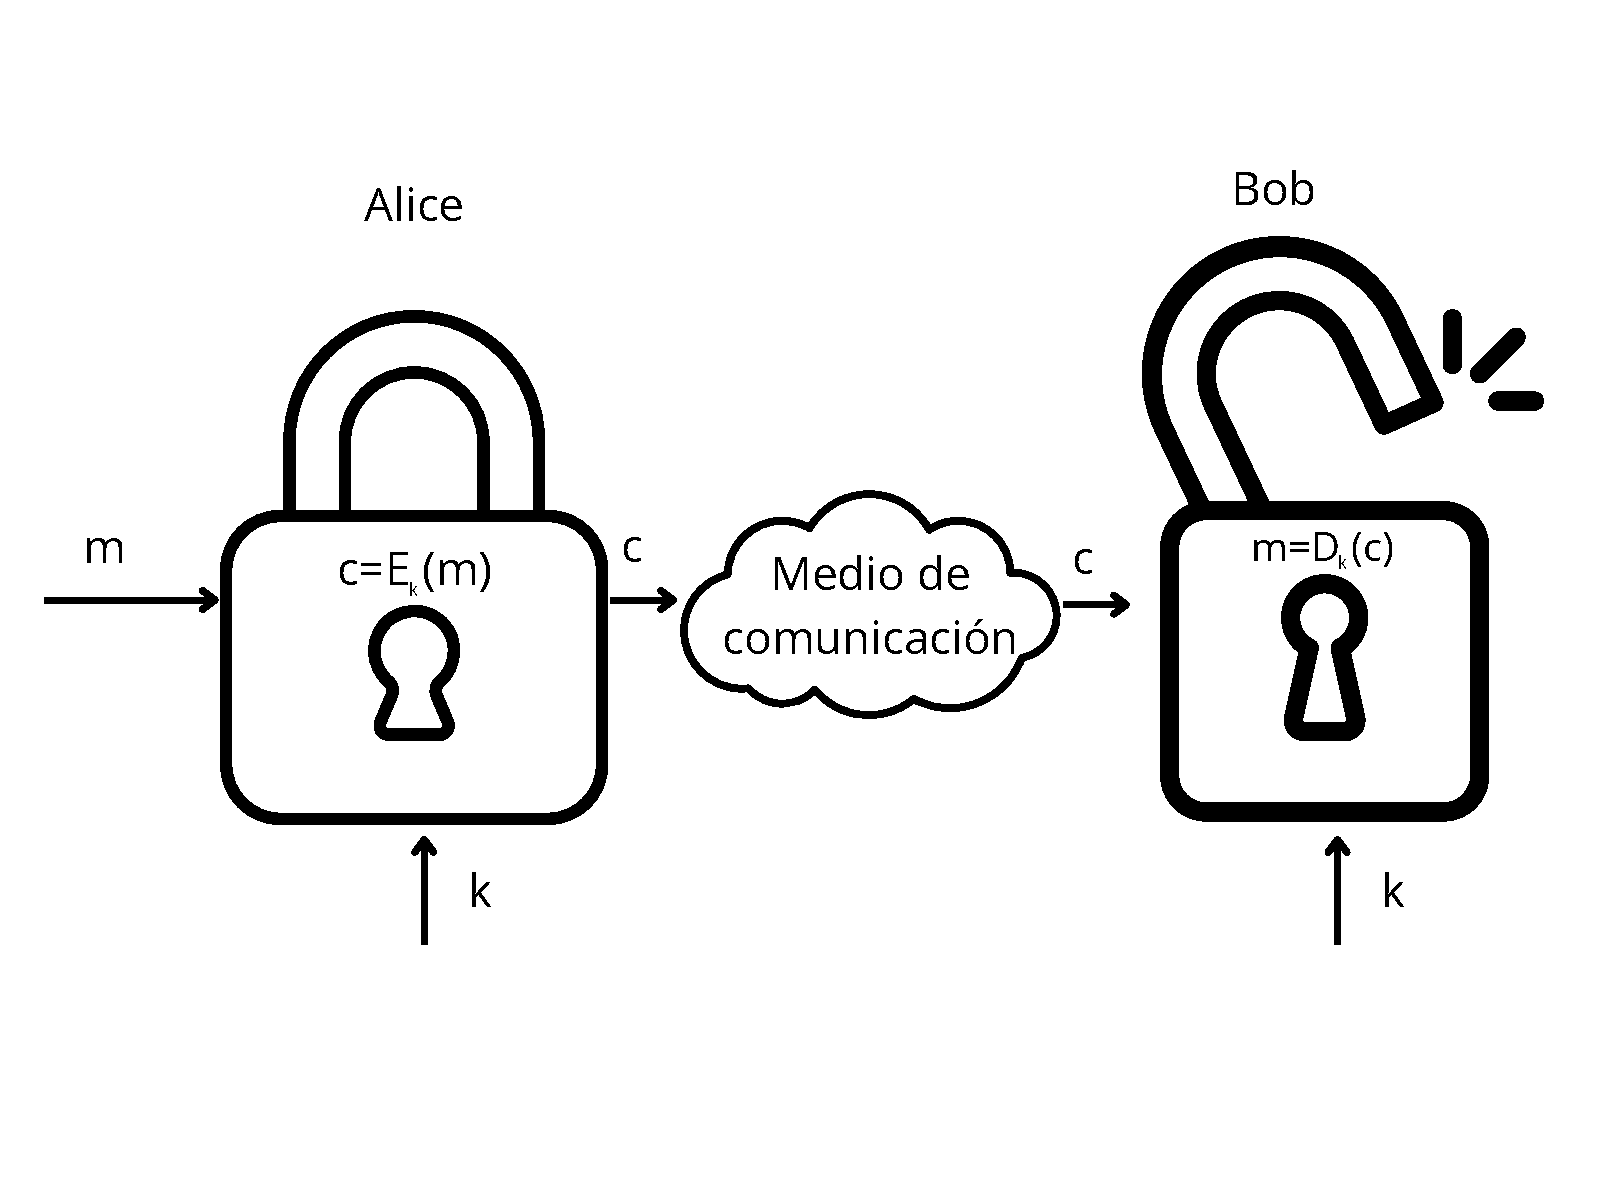
\includegraphics[width = 0.7\textwidth]{Imagenes/pitea/clave_secreta.pdf}
	\caption[Diagrama criptografía de clave secreta.]{Diagrama criptografía de clave secreta. Elaboración propia.}
	\label{fig:clave_secreta}
\end{figure}

Como se puede apreciar en la figura~\ref{fig:clave_secreta}, denominamos ``$m$'' al mensaje en claro, ``$c$'' al mensaje cifrado y ``$k$'' a la clave secreta. El proceso de cifrado se define mediante la función:
\[
c = E_k(m)
\]
donde \( E_k \) es el algoritmo de cifrado, que a partir del mensaje en claro y una clave secreta, genera el mensaje cifrado. Ambos mensajes pueden representarse en diferentes formatos, tales como secuencias de bits, números, cadenas de texto o cualquier otro tipo de dato compatible con las operaciones internas de la función de cifrado.\\
De manera análoga, el proceso de descifrado se describe mediante la función:
\[
m = D_k(c)
\]
en la que \( D_k \) representa el algoritmo de descifrado. Este recibe como entrada el mensaje cifrado y, utilizando la misma clave secreta ``$k$'', recupera el mensaje original. Considerando los tipos de datos, el método de descifrado funciona de manera inversa al cifrado, intercambiando los tipos de entrada y salida.\\

Uno de los ejemplos más antiguos de este tipo de cifrado es el cifrado ``César'', el cual debe su nombre a que fue uno de los principales métodos de cifrado del imperio romano. Se trata de un algoritmo de cifrado por sustitución, como se puede apreciar en la figura~\ref{fig:cesar}, donde cada carácter es reemplazado por otro. Su algoritmo de cifrado es descrito como: 
\[
c[i] = (m[i] + k)  \mod  \,N  
\]
siendo $m[i]$ el carácter en la posición $i$ del mensaje, $c[i]$ el resultado en el mensaje cifrado en la misma posición y $N$ el tamaño del alfabeto ($\Sigma$). Su función de descifrado es:
\[
m[i] = (c[i] - k)  \mod  \,N 
\]
cumpliéndose que todos los componentes de los mensajes en claro y cifrados pertenezcan al alfabeto :
\[
\forall r \in m, \, r \in \Sigma \quad \text{y} \quad \forall g \in c, \, g \in \Sigma \, .
\]



    \begin{figure}[h]
	\centering
	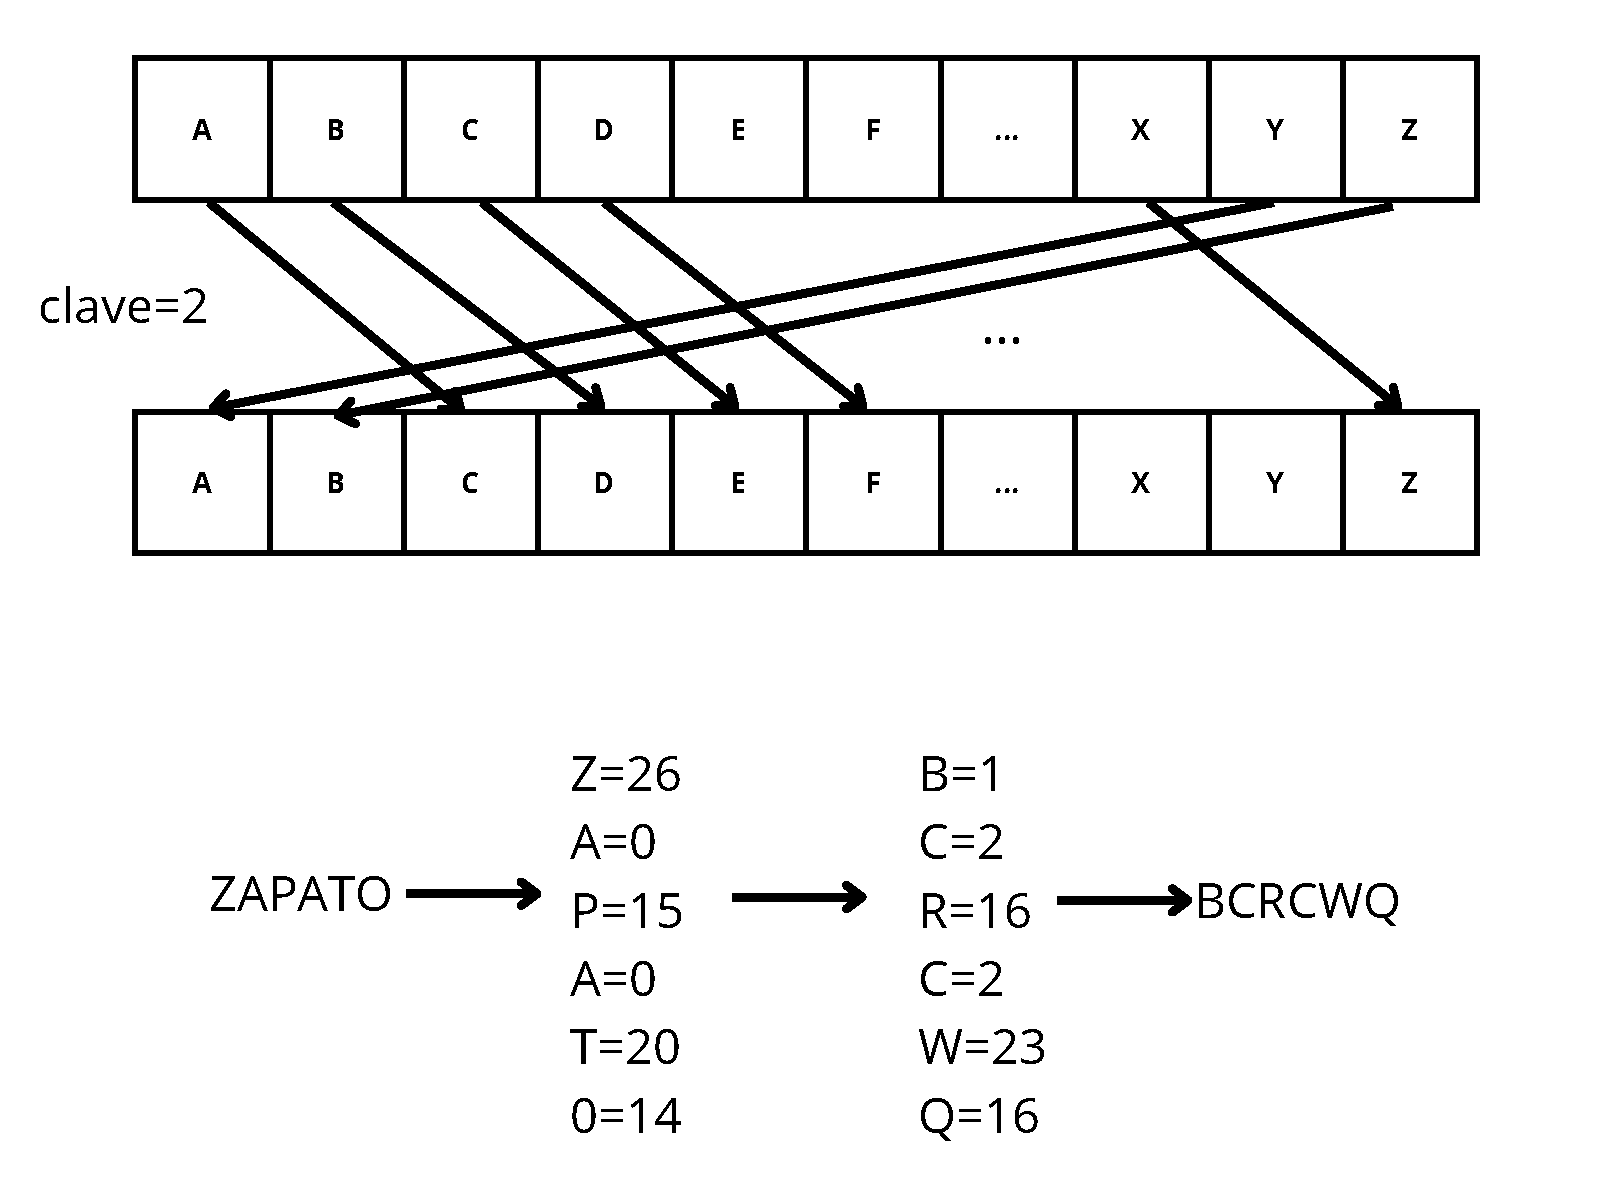
\includegraphics[width = 0.7\textwidth]{Imagenes/pitea/cesar.pdf}
	\caption[Ejemplo cifrado César.]{Ejemplo cifrado César. Elaboración propia.}
	\label{fig:cesar}
\end{figure}


Volviendo a tiempos más modernos está el cifrador AES (\textit{Advanced Encryption Standard})\footnote{\cite{NISTFIPS197}}, para el cual se seleccionó el algoritmo de Rijndael, de los criptógrafos belgas  Joan Daemen y Vincent Rijmen, en el año 2001 tras el concurso realizado por el NIST (\textit{National Institute of Standards and Technology}). El concurso fue lanzado en septiembre de 1997, con el fin de recibir nuevas propuestas de algoritmos de protección de información tanto civil como militar.\\

El algoritmo de Rijndael se lleva a cabo mediante el siguiente proceso:

\begin{itemize}
  \item \textbf{Primera ronda}: 
    \begin{itemize}
     \item Adición de la clave de ciclos (\textit{AddRoundKey}).
     \end{itemize}
  \item \textbf{N rondas básicas}: figura~\ref{fig:aes}, cada una compuesta por:
  \begin{itemize}
    \item Sustitución de bytes (\textit{ByteSub}).
    \item Desplazamiento de filas (\textit{ShiftRow}).
    \item Mezcla de columnas (\textit{MixColumns}).
    \item Adición de la clave de ciclos (\textit{AddRoundKey}).
  \end{itemize}
  \item \textbf{Ronda final}:
  \begin{itemize}
    \item Sustitución de bytes.
    \item Desplazamiento de filas. 
    \item Adición de la clave de ciclos.
  \end{itemize}
\end{itemize}


    \begin{figure}[h]
	\centering
	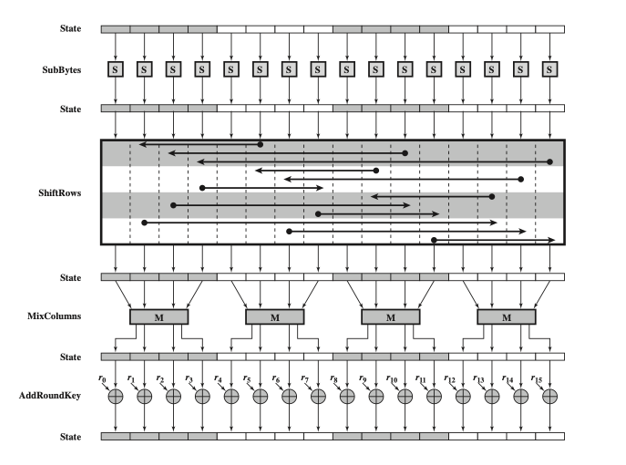
\includegraphics[width = 0.7\textwidth]{Imagenes/pitea/aes.png}
	\caption[Ciclo básico del algoritmo de Rijndael.]{Ciclo básico del algoritmo de Rijndael,~\cite{Stallings2022}.}
	\label{fig:aes}
\end{figure}

A continuación se hablará de cada una de las funciones mencionadas en las etapas del algoritmo de Rijndael:

\begin{enumerate}
  \item\label{sec:subBytes} Sustitución de bytes:\\
  
  Se trata de una sustitución no lineal que se realiza sobre todos los bytes; esta sustitución se conforma de dos etapas: 
  \begin{enumerate}
        \item Cada byte se sustituye por su inverso multiplicativo (considerándose cada uno un elemento del conjunto $GF(2^8)$~\footnote{\url{Http://www.math.huji.ac.il/\textasciitilde jgutierrez/GaloisFinitos.pdf}.})
        y el 00 por sí mismo.
        \item A la salida de la sustitución anterior se le aplica la siguiente operación:
            \[
            \begin{pmatrix}
            y_0 \\ y_1 \\ y_2 \\ y_3 \\ y_4 \\ y_5 \\ y_6 \\ y_7
            \end{pmatrix}
            =
            \begin{pmatrix}
            1 & 0 & 0 & 0 & 1 & 1 & 1 & 1 \\
            1 & 1 & 0 & 0 & 0 & 1 & 1 & 1 \\
            1 & 1 & 1 & 0 & 0 & 0 & 1 & 1 \\
            1 & 1 & 1 & 1 & 0 & 0 & 0 & 1 \\
            1 & 1 & 1 & 1 & 1 & 0 & 0 & 0 \\
            0 & 1 & 1 & 1 & 1 & 1 & 0 & 0 \\
            0 & 0 & 1 & 1 & 1 & 1 & 1 & 0 \\
            0 & 0 & 0 & 1 & 1 & 1 & 1 & 1 \\
            \end{pmatrix}
            \cdot
            \begin{pmatrix}
            x_0 \\ x_1 \\ x_2 \\ x_3 \\ x_4 \\ x_5 \\ x_6 \\ x_7
            \end{pmatrix}
            +
            \begin{pmatrix}
            0 \\ 1 \\ 1 \\ 0 \\ 0 \\ 0 \\ 1 \\ 1
            \end{pmatrix}.
            \]

\end{enumerate}
  \item Desplazamiento de filas:\\
  
   Se desplazan cíclicamente a la izquierda las filas; el número de veces que se desplaza cada fila depende de su posición\footnote{\citep[p. 17]{NISTFIPS197} .}. 
   \[
s'_{r,c} = s_{r, (c + r) \bmod 4}, \quad \text{para } 0 \leq r < 4, \; 0 \leq c < 4 
\]

siendo $S_{r,c}$ el byte en la fila $r$ y columna $c$.

  \item Mezcla de columnas:\\

  Cada byte constituyente de cada columna de la salida de la función anterior es representado como polinomio sobre $GF(2^8)$ y multiplicado por un polinomio constante $c(x)$ módulo $x^4+1$.

  \[
c(x)= 03_{16} x^3+01_{16}x^2+01_{16}x+02_{16}.
  \]
  \item Adición de la clave de ciclos:\\

  Se aplica la operación XOR a la salida de la función anterior y a la subclave correspondiente.

  Estas subclaves son expansiones del mismo tamaño que la original. Estas expansiones consisten en añadir 4 bytes obtenidos al aplicar XOR entre la clave y partes predeterminadas de la expansión anterior. La primera vez, se realiza a la clave la sustitución de bytes, explicada anteriormente en el punto 1 de esta enumeración, y se aplica XOR con una constante definida en función del número del ciclo.

\end{enumerate}

\FloatBarrier  % Evita que la imagen pase más allá de este punto
\subsection{Criptografía de clave pública }
A diferencia de la criptografía de clave secreta, en la criptografía de clave pública no se cifra y descifra con la misma clave, sino que se utiliza una clave para cifrar y otra para descifrar, por eso también es llamada criptografía asimétrica. Cuando hablamos de clave en este tipo de criptosistema nos referimos a un par de claves, la clave secreta $KS$, la cual se debe mantener protegida, y la clave pública $KP$, la cual puede viajar por la red sin protección ninguna. Este par de claves debe cumplir que la clave pública sea fácilmente derivable de la clave privada pero que la privada sea computacionalmente impracticable obtenerla a partir de la clave pública.\\

Como se puede ver en la figura ~\ref{fig:publica}, si se desea mandar un mensaje cifrado a un usuario o sistema \textbf{B}, se adquiere su clave pública, la cual puede viajar sin protección al no poner en riesgo la confidencialidad de los mensajes posteriormente cifrados por ella y se cifra el mensaje que se desea que únicamente pueda leer \textbf{B}. Al recibir el mensaje cifrado, \textbf{B} lo descifra con su clave secreta.\\

    \begin{figure}[h]
	\centering
	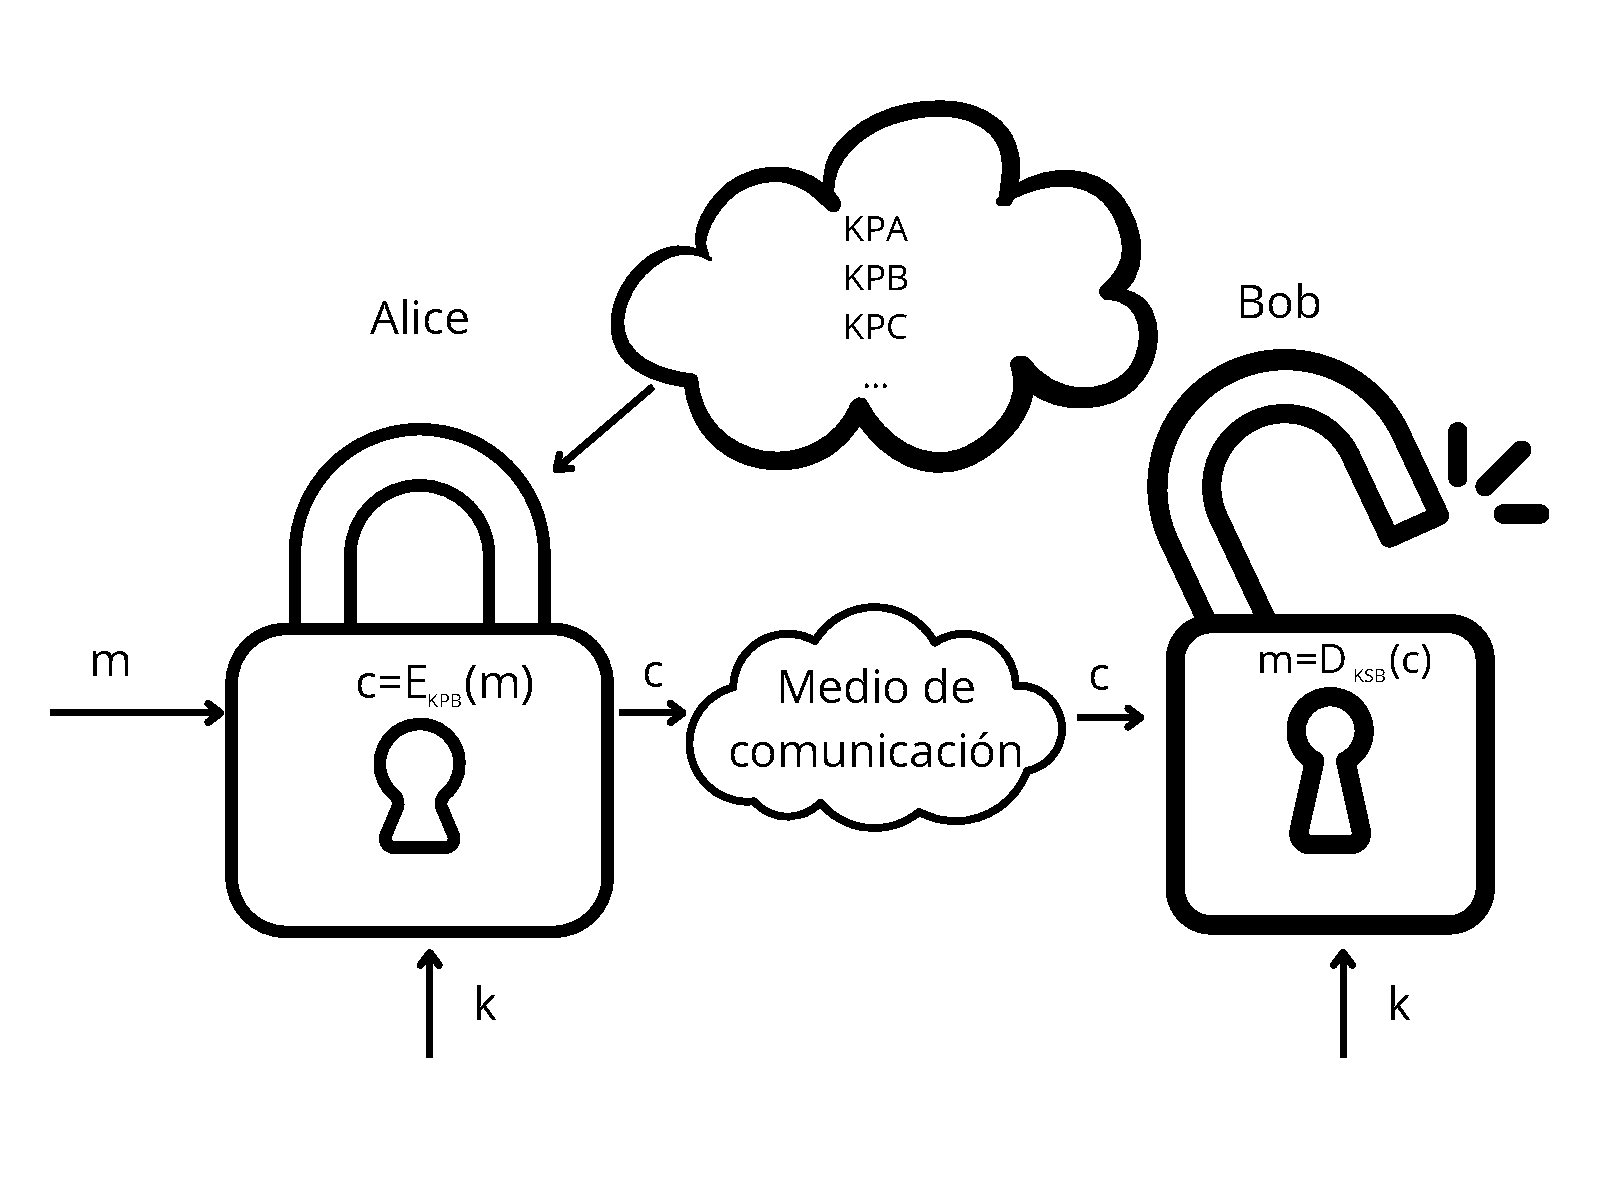
\includegraphics[width = 0.7\textwidth]{Imagenes/pitea/clave_publica.pdf}
	\caption[Diagrama criptografía de clave pública.]{Diagrama criptografía de clave pública. Elaboración propia.}
	\label{fig:publica}
\end{figure}


Además de la capacidad de cifrar mensajes, la criptografía de clave pública permite el firmado de mensajes, mediante el cifrado con la clave secreta y descifrado con la clave pública de un \textit{hash} del mensaje; esto proporciona integridad y autenticidad de los datos. Esto se debe a que, si bien el mensaje puede ser visto por cualquiera, solo se puede hacer utilizando la clave pública de la entidad que ha cifrado el mensaje con su clave secreta, figura~\ref{fig:firma}.

    \begin{figure}[h]
	\centering
	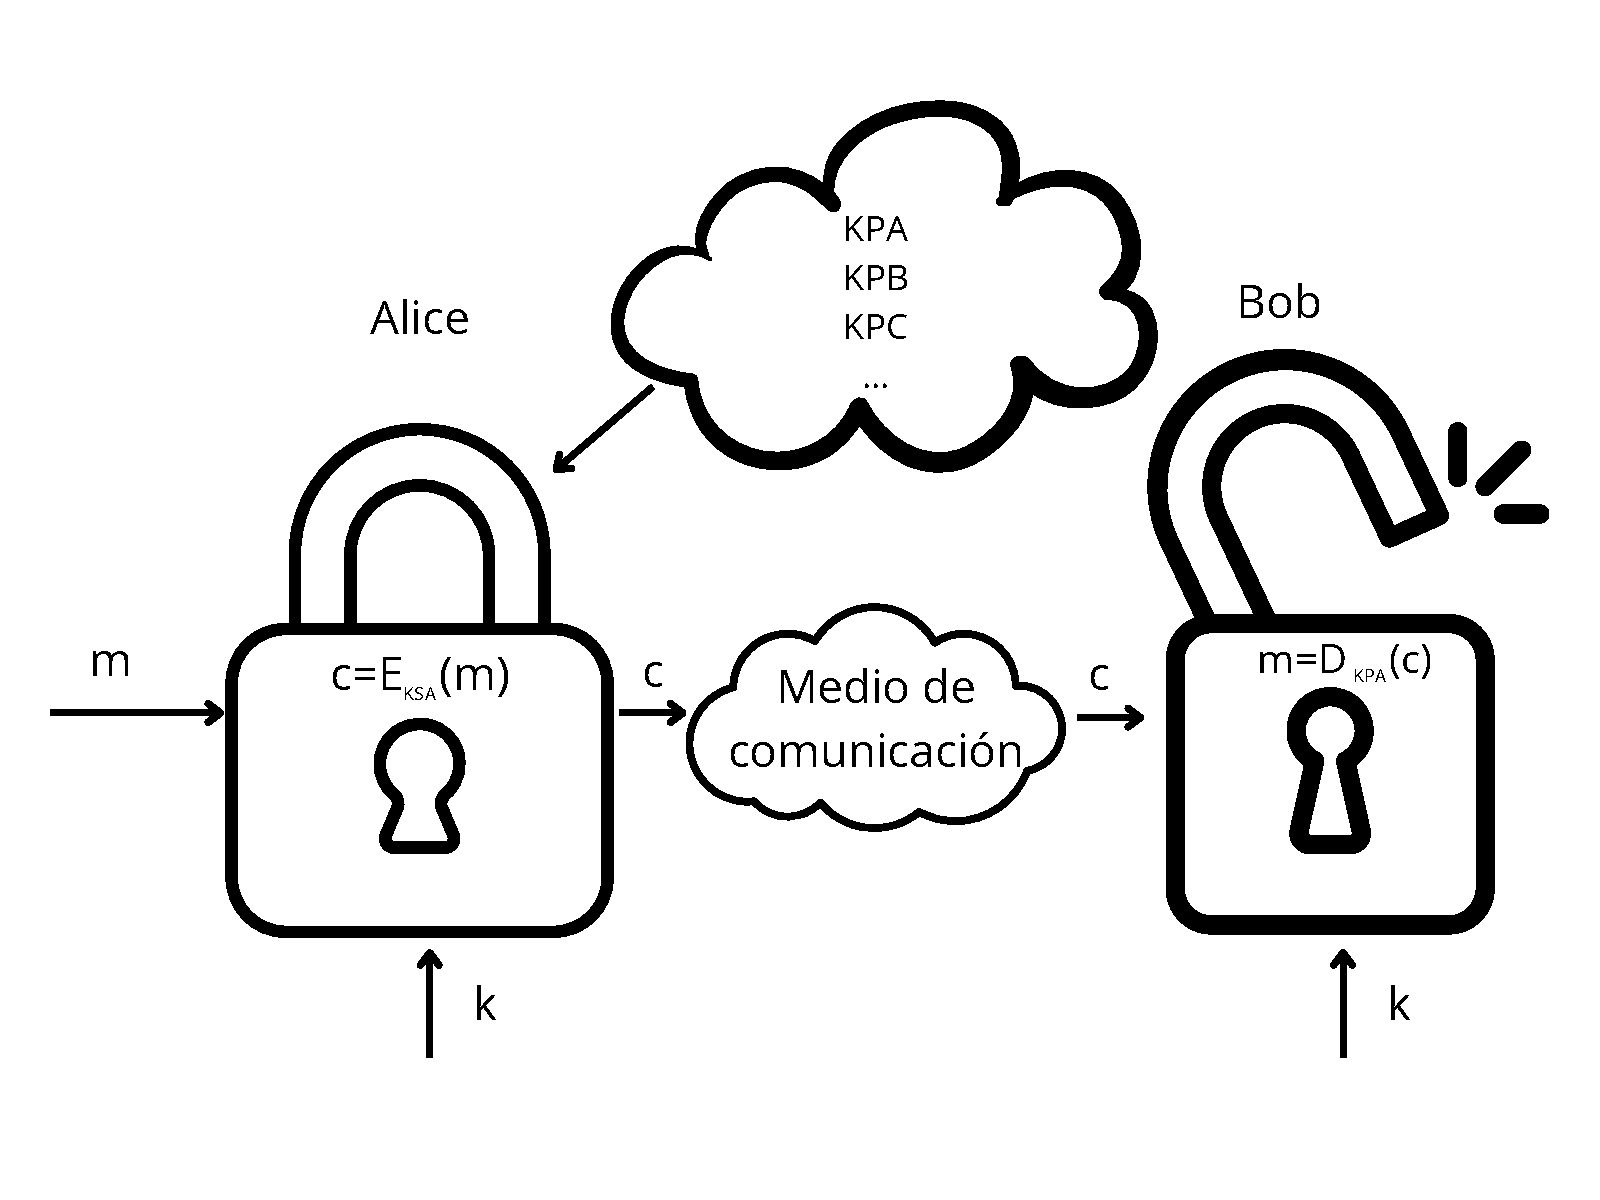
\includegraphics[width = 0.7\textwidth]{Imagenes/pitea/firma.pdf}
	\caption[Firmado con clave pública.]{Firmado con clave pública. Elaboración propia.}
	\label{fig:firma}
\end{figure}
\FloatBarrier  % Evita que la imagen pase más allá de este punto

Uno de los algoritmos más conocidos de este tipo de criptosistemas es el RSA\footnote{\cite{NISTSP80056BRev2}.}, cuyo nombre está compuesto de las iniciales de sus creadores: Rivest, Shamir y Adleman.\\

El RSA afronta el cifrado de manera diferente al AES, ya que en este caso el mensaje se divide en bloques de forma que el valor de los bloques sean números enteros que cumplan: \[0< \text{valor de bloque} <n-1 \,  \text{y} \, \text{número de bits de cada bloque} <=  log_2 (n).\]

 \begin{enumerate}
    \item Generación de claves:
        \begin{enumerate}
            \item Se eligen dos números primos $p$ y $q$~\footnote{Para asegurar la seguridad del algoritmo hoy en día es necesario que tengan un tamaño superior a 100 dígitos en base 10 y ambos números sean de un tamaño parecido.}.
            \item Se calcula:
            \[n= p*q.\]
            \item Se elige un $e$ tal que:
            \[\operatorname{mcd}(e,\varphi(n)) = 1 \mod n\]
            siendo $\varphi(n)$ la función de Euler,\[
\varphi(n) = \#\left\{ k \in \mathbb{Z} \,\middle|\, 1 \leq k \leq n,\ \operatorname{mcd}(k, n) = 1 \right\}
\]

la cantidad de números enteros menores de $n$ que son coprimos con $n$, además sabemos que: \[p, q \text{ primos} \Rightarrow \varphi(p*q) = (p - 1)(q - 1).\]
            \item Se calcula $d$ de forma que:
            \[d=e^{-1} \mod \varphi(n)\]

            
            siendo $KP=\{n,e\}$ y $KS=\{n,d\}$.
         \end{enumerate}
    \item Cifrado y descifrado.
    \begin{itemize}
    \item Cifrado:
    \[c=m^e \mod n.\]
    \item Descifrado
    \[m=c^d \mod n.\]
    \end{itemize}
 \end{enumerate}


La seguridad del algoritmo se basa en que el cálculo de $\varphi(n)$ sin conocer $p$ y $q$ es computacionalmente inviable, debido a que no conocemos ningún algoritmo con una eficiencia polinómica o menor.



\section{Transmisión de datos mediante SSTV}
En esta sección se hablará de qué es SSTV y de su funcionamiento básico, ya que para el fin de la herramienta no es necesario profundizar en detalles técnicos ni en los detalles particulares de cada uno de los 27 modos de transmisión.\\

Según~\cite{IARUEtica}, SSTV (\textit{Slow Scan Television} o en español, Televisión de barrido lento) es un modo de transmisión capaz de recibir y transmitir imágenes estáticas vía radio. Este modo de transmisión utiliza un ancho de banda máximo de \SI{2.7}{\kilo\hertz} aproximadamente, siendo representado el negro por un tono a \SI{1500}{\hertz} y \SI{2300}{\hertz}  para el blanco. Además se une un pulso sincronizado (sync pulse) en \SI{1200}{\hertz} de manera que al ser bastante inferior al negro es invisible. Estos pulsos se envían al final de cada línea, durando \SI{5}{\milli\second}, y al final de cada imagen con una duración de \SI{30}{\milli\second}. Siendo su función mantener sincronizado el receptor con el transmisor, garantizando que la imagen se reconstruya correctamente, figura~\ref{fig:Onda_sstv_b_n}.\\
    \begin{figure}[h]
	\centering
	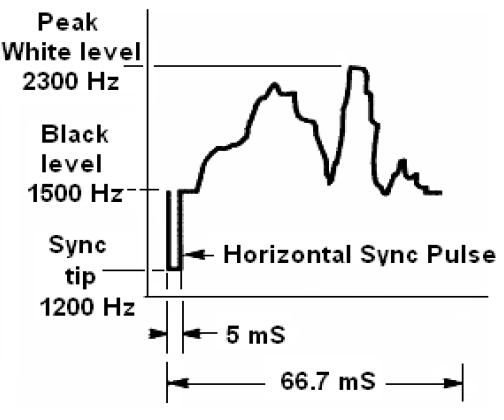
\includegraphics[width = 0.5\textwidth]{Imagenes/pitea/Onda_sstv_b_n.png}
	\caption[Onda de audio usando SSTV para imágenes en blanco y negro.]{Onda de audio usando SSTV para imágenes en blanco y negro,~\cite{IARUEtica}.}
	\label{fig:Onda_sstv_b_n}
\end{figure}

\begin{figure}[h]
	\centering
	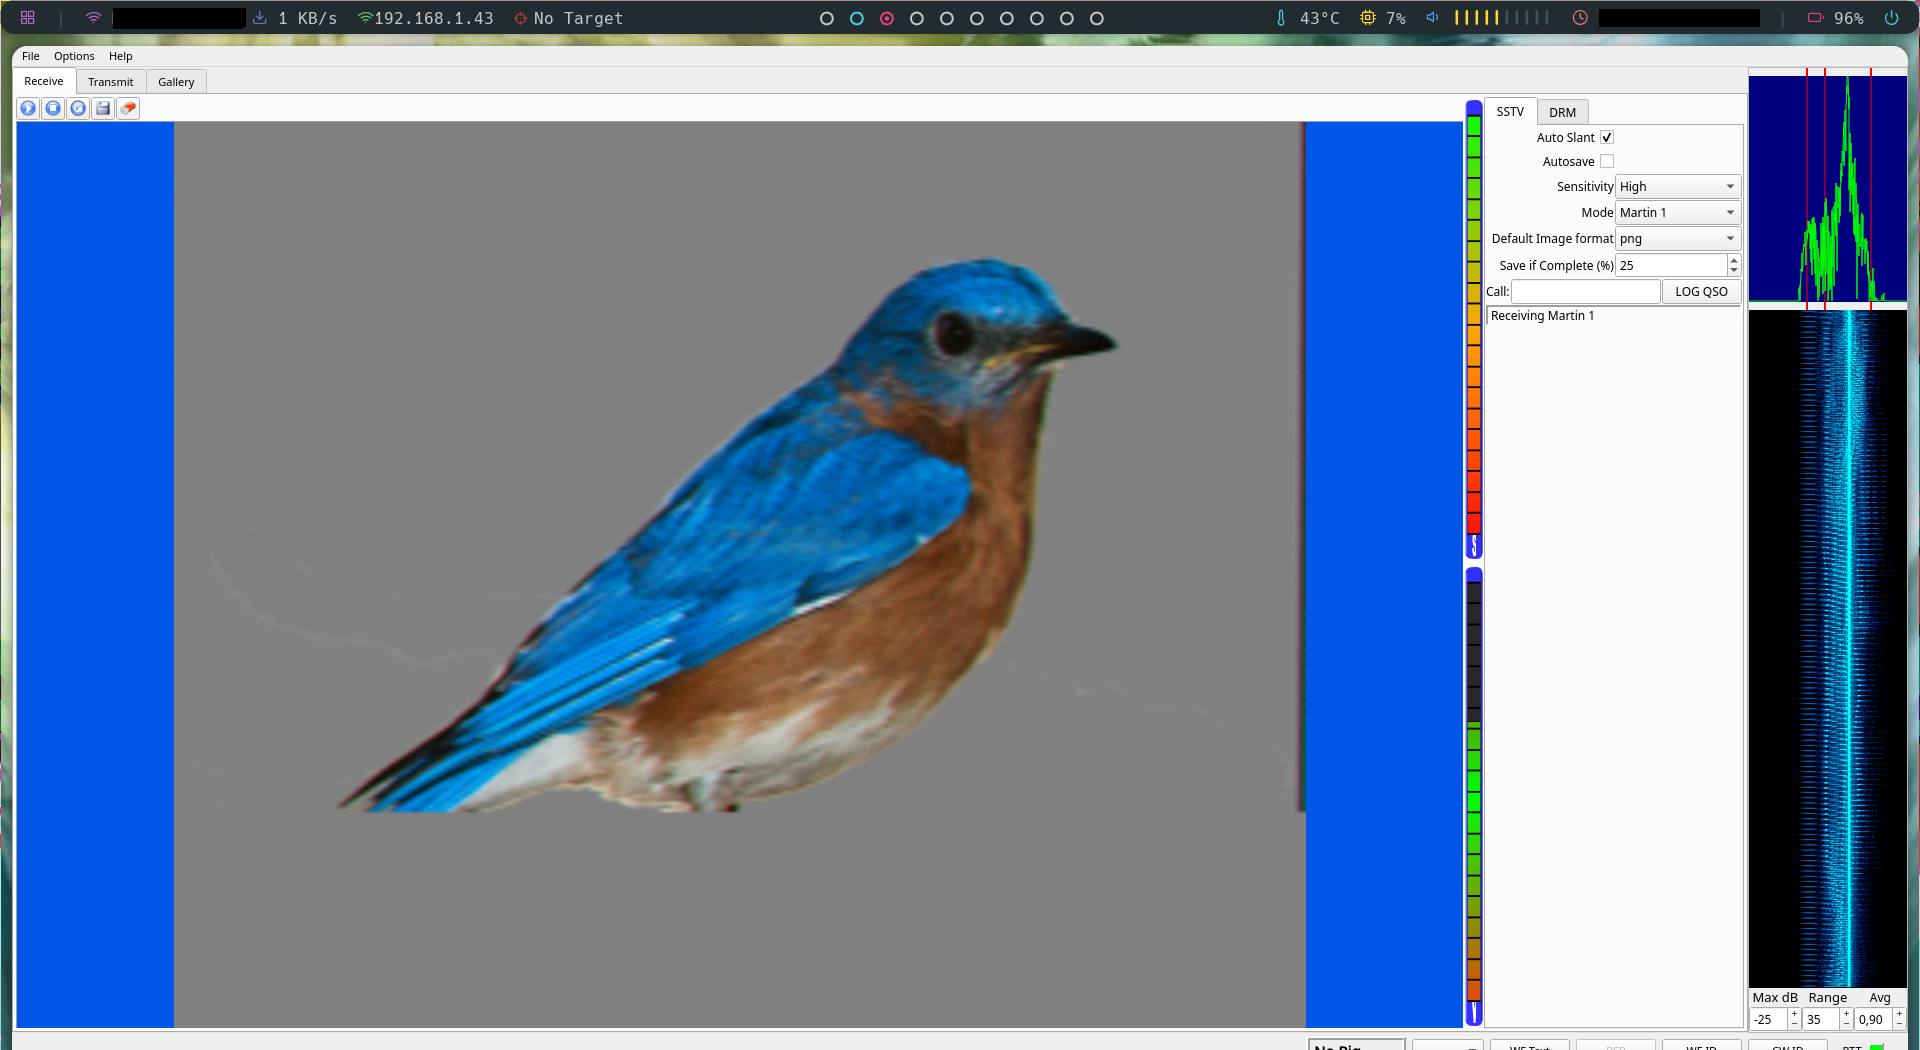
\includegraphics[width = 0.6\textwidth]{Imagenes/pitea/pajaro.png}
	\caption[Decodificación de un audio en SSTV usando QSSTV.]{Decodificación de un audio en SSTV usando QSSTV. Elaboración propia.}
	\label{fig:proceso}
\end{figure}

SSTV utiliza modulación de frecuencia, asociando una frecuencia de audio distinta a cada distinto valor de intensidad ubicable en los diferentes puntos de la imagen. Los colores son conseguidos enviando la intensidad de cada componente RGB de manera separada y consecutiva.\\

En la tabla~\ref{tab:SSTVBandas} se pueden observar las frecuencias más usadas por radioaficionados para transmisión por SSTV, significando LSB (solo en esta sección), \textit{Lower Side Band} y USB, \textit{Upper Side Band}.

\begin{table}[h]
	\centering
	\begin{tabular}{c|c|c}
		\textbf{Banda} & \textbf{Frecuencia} & \textbf{Modo} \\
		\hline\hline
		80 m  & \SI{3735 \pm 5}{\kilo\hertz}                 & LSB \\
		40 m  & \SIrange{7035}{7050}{\kilo\hertz}         & LSB \\
		20 m  & \SIrange{14220}{14235}{\kilo\hertz}         & USB \\
		15 m  & \SIrange{21330}{21346}{\kilo\hertz}         & USB \\
		10 m  & \SIrange{28670}{28690}{\kilo\hertz}         & USB \\
		\hline
	\end{tabular}
	\caption[Frecuencias típicas para transmisión SSTV.]{Frecuencias típicas de uso para SSTV en bandas de radioaficionado,~\cite{IARUEtica}.}
	\label{tab:SSTVBandas}
\end{table}

\FloatBarrier

\section{Comparación con otras herramientas}

En esta sección se comparará la herramienta desarrollada con otras herramientas muy usadas del mundo de la esteganografía, como \textit{Steghide}\footnote{\url{Https://steghide.sourceforge.net/} .} y \textit{SilentEye}\footnote{\url{Https://github.com/achorein/silenteye} .}. \\

\textit{Steghide} es una de las herramientas más conocidas en el mundo de la esteganografía, esta viene instalada por defecto en las distribuciones de \textit{Kali Linux}. \textit{Steghide} permite ocultar datos en archivos de imagen en los formatos JPEG, BMP (\textit{Bits Maps Protocole}) y también de audio en formatos WAV y AU (\textit{Audio file format}). La característica más relevante de \textit{Steghide} es que oculta información sin producir cambios visibles en los tonos de color o en las propiedades de muestreo del archivo original, logrando así que sea resistente a pruebas estadísticas de primer orden, este tipo de pruebas evalúa la frecuencia de aparición de cada símbolo (por ejemplo, unos y ceros en una secuencia binaria) y la compara con la distribución teórica esperada mediante tests como el chi-cuadrado o medidas de entropía para detectar desviaciones. Además, dispone de funcionalidades como la compresión de datos antes de ocultarlos, la protección del contenido con un cifrado robusto e incorpora también un mecanismo para comprobar posteriormente que la información recuperada no ha sido modificada. A continuación, se pueden ver en la figura \ref{fig:steghide} unos ejemplos de uso de \textit{Steghide}.\\

\begin{figure}[h]
	\centering
	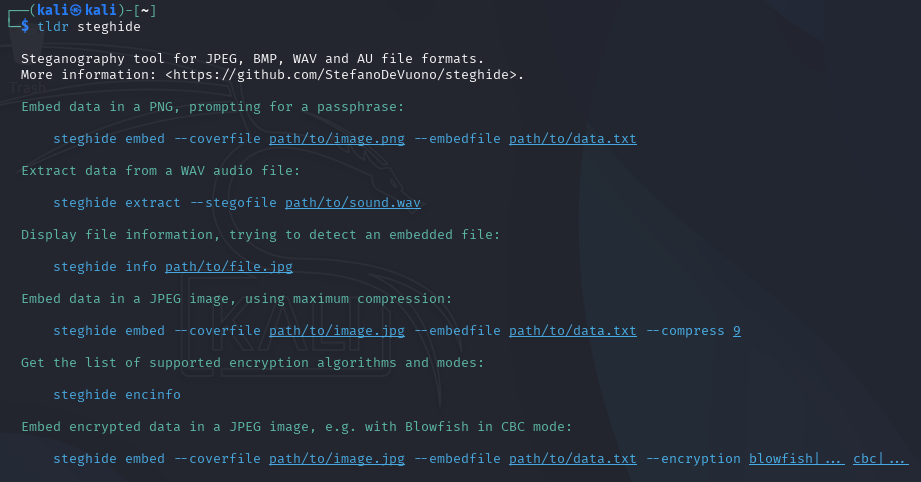
\includegraphics[width = 1\textwidth]{Imagenes/steghide.png}
	\caption[Ejemplos de uso de \textit{Steghide}.]{Ejemplos de uso proporcionado por tldr  de \textit{Steghide}.}
        \caption*{{\url{Https://tldr.sh/}, tldr es una herramienta que muestra páginas de ayuda que han sido creadas por la comunidad para simplificar las páginas del manual mediante ejemplos prácticos.}}
	\label{fig:steghide}
    \end{figure}
    \FloatBarrier

\textit{Steghide} es muy buena ocultando información en imágenes y audio usando LSB, pero tiene limitaciones claras.  PITEA no solo hace ocultaciones mediante LSB en PNG y en WAV, sino que también añade otras opciones, como generar una imagen  directamente con la información cifrada y codificada en base64, algo que \textit{Steghide} no puede hacer. Otra ventaja de PITEA es la posibilidad de modular una señal de audio para SSTV a partir de una imagen con texto incrustado en ella. Esto permite que la imagen se pueda transmitir por radiofrecuencia y el mensaje oculto pueda ser recuperado posteriormente. Como veremos más adelante, si el secreto estuviera oculto en la imagen mediante LSB, este no podría ser recuperado.
\\

\textit{SilentEye}, también oculta mediante LSB en archivos en formato JPEG, BMP y WAV, dispone de cifrado con AES128 o AES256, dispone de compresión zlib\footnote{zlib es una biblioteca de compresión sin pérdida basada en el algoritmo DEFLATE.} para reducir el tamaño del mensaje antes de incrustarlo y de un sistema de  \textit{plugins} que permite la integración de manera sencilla de nuevos algoritmos de esteganografía o procesos de criptografía. En las figuras \ref{fig:silenteye1} y \ref{fig:silenteye2} se puede observar la pantalla de inicio de \textit{SilentEye} y las opciones que son desplegadas al seleccionar la opción de encode. \\

\textit{SilentEye}, tampoco implementa la generación de una imagen directamente con el texto cifrado y codificado en base64, ni la posibilidad de transformar la imagen generada en una señal SSTV. Además, debido a que PITEA está desarrollada teniendo en cuenta los patrones de diseño GoF (\textit{Gang of Four})  es sencillo añadir nuevos tipos de cifrado o métodos de ocultación si se tienen conocimientos básicos de POO (Programación Orientada a Objetos).



    \begin{figure}[h]
	\centering
	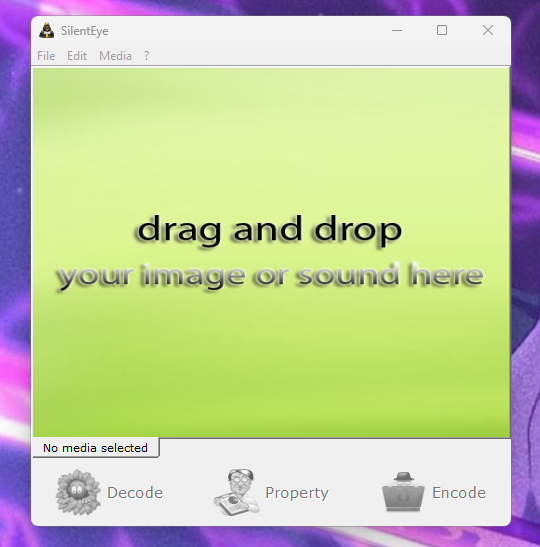
\includegraphics[width = 0.5\textwidth]{Imagenes/silenteye1.png}
	\caption[Pantalla de inicio de \textit{SilentEye}.]{Pantalla de inicio de \textit{SilentEye}. Captura de pantalla.}
	\label{fig:silenteye1}
    \end{figure}

    \begin{figure}[h]
	\centering
	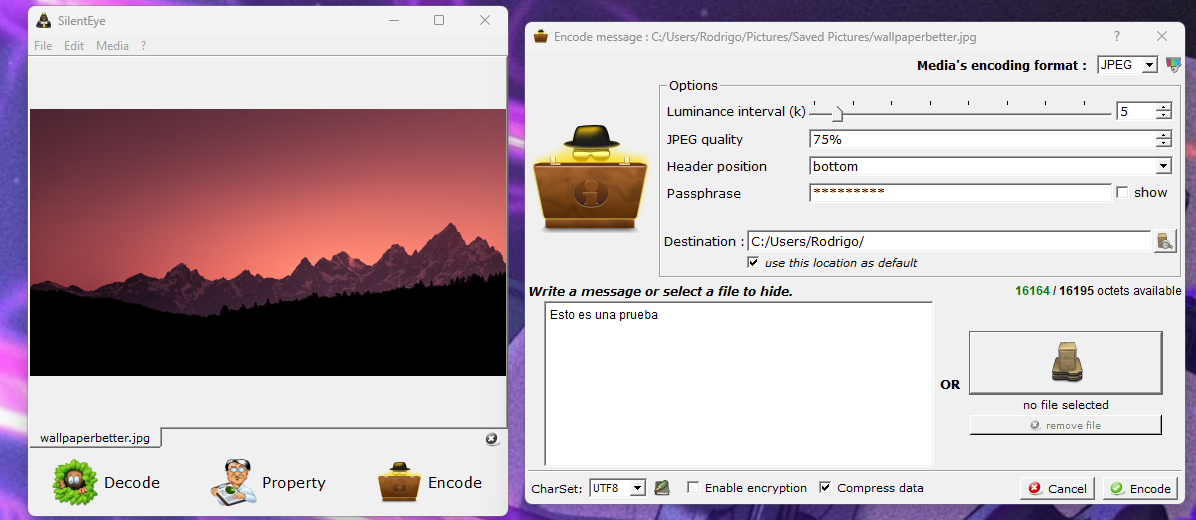
\includegraphics[width = 1\textwidth]{Imagenes/silenteye2.png}
	\caption[Menú \textit{encode} de \textit{SilentEye}.]{Menú \textit{encode} de \textit{SilentEye}. Captura de pantalla.}
	\label{fig:silenteye2}
    \end{figure}











